\documentclass[sigconf]{acmart}

\newcommand{\FIXME}[1]{{\color{red}{\textbf{FIXME:}#1}}}

\usepackage{booktabs} % For formal tables

% Copyright
%\setcopyright{none}
%\setcopyright{acmcopyright}
%\setcopyright{acmlicensed}
\setcopyright{rightsretained}
%\setcopyright{usgov}
%\setcopyright{usgovmixed}
%\setcopyright{cagov}
%\setcopyright{cagovmixed}


% DOI
\acmDOI{10.475/123_4}

% ISBN
\acmISBN{123-4567-24-567/08/06}

%Conference
\acmConference[SHORTNAME'17]{ACM Long Conference Name conference}{July 1997}{City, State, Country} 
\acmYear{2017}
\copyrightyear{2017}

\acmPrice{15.00}

\usepackage{xspace}
\newcommand{\OurSys}{Wharf\xspace}

\usepackage{algorithm2e}

\begin{document}
\title{In-network computing to the rescue of faulty links}
%\title{SIG Proceedings Paper in LaTeX Format}
%\titlenote{Produces the permission block, and copyright information}
%\subtitle{Extended Abstract}

\author{Anirudh Chelluri \kern1em
 Andr\'e DeHon \kern1em
 Hans Giesen \kern1em
 Boon Thau Loo \kern1em
 Nishanth Prabhu \kern1em
 Lei Shi \kern1em
 John Sonchack \kern1em
 Nik Sultana}
\affiliation{%
\institution{University of Pennsylvania}}

%\author{Firstname Lastname}
%\authornote{Note}
%\orcid{1234-5678-9012}
%\affiliation{%
%  \institution{Affiliation}
%  \streetaddress{Address}
%  \city{City} 
%  \state{State} 
%  \postcode{Zipcode}
%}
%\email{email@domain.com}
%
%\author{Firstname Lastname}
%\orcid{1234-5678-9012}
%\affiliation{%
%  \institution{Affiliation}
%  \streetaddress{Address}
%  \city{City} 
%  \state{State} 
%  \postcode{Zipcode}
%}
%\email{email@domain.com}
%
%\author{Firstname Lastname}
%\orcid{1234-5678-9012}
%\affiliation{%
%  \institution{Affiliation}
%}
%\email{email@domain.com}
%
%\author{Firstname Lastname}
%\orcid{1234-5678-9012}
%\affiliation{%
%  \institution{Affiliation}
%}
%\email{email@domain.com}
%
%\author{Firstname Lastname}
%\orcid{1234-5678-9012}
%\affiliation{%
%  \institution{Affiliation}
%}
%\email{email@domain.com}


% The default list of authors is too long for headers}
%\renewcommand{\shortauthors}{F. Lastname et al.}
\renewcommand{\shortauthors}{A. Chelluri et al.}

\begin{abstract}
Failing network links are usually disabled, and packets are routed around them
until the links are repaired.  But it is often possible
to utilise some of a failing link's capacity. Losing what remains of a link's
capacity is deemed preferable to the erratic effect that unreliable links can
have on application-level behaviour.

We describe a new network function that relies on in-network computing to limit
the erratic effect of failing network links, to enable the continued use of
those links until they can be repaired. We argue that such a network function
can help mitigate rolling failures in datacenter networks, and that our design
can interoperate with existing network architecture and configuration choices,
such as for multi-path routing.

We model our design using ns-3, and evaluate our implementation on a physical
test-bed that includes programmable switches and reconfigurable hardware.
\end{abstract}

%
% The code below should be generated by the tool at
% http://dl.acm.org/ccs.cfm
% Please copy and paste the code instead of the example below. 
%
\begin{CCSXML}
<ccs2012>
 <concept>
  <concept_id>10010520.10010553.10010562</concept_id>
  <concept_desc>Computer systems organization~Embedded systems</concept_desc>
  <concept_significance>500</concept_significance>
 </concept>
 <concept>
  <concept_id>10010520.10010575.10010755</concept_id>
  <concept_desc>Computer systems organization~Redundancy</concept_desc>
  <concept_significance>300</concept_significance>
 </concept>
 <concept>
  <concept_id>10010520.10010553.10010554</concept_id>
  <concept_desc>Computer systems organization~Robotics</concept_desc>
  <concept_significance>100</concept_significance>
 </concept>
 <concept>
  <concept_id>10003033.10003083.10003095</concept_id>
  <concept_desc>Networks~Network reliability</concept_desc>
  <concept_significance>100</concept_significance>
 </concept>
</ccs2012>  
\end{CCSXML}

\ccsdesc[500]{Computer systems organization~Embedded systems}
\ccsdesc[300]{Computer systems organization~Redundancy}
\ccsdesc{Computer systems organization~Robotics}
\ccsdesc[100]{Networks~Network reliability}

% We no longer use \terms command
%\terms{Theory}

\keywords{ACM proceedings}


\maketitle

\section{Introduction}

In this paper we describe \OurSys, an in-network distributed mitigation for
faulty links.  We claim that our design requires minimal configuration, is
transparent to end-points~\cite{Saltzer84end-to-endarguments} and does not
conflict with existing network architecture choices (e.g., what topology to use
and how to route over it). We model \OurSys using ns-3 and evaluate
implementations for CPUs and FPGAs.


\begin{figure}
  \centering
  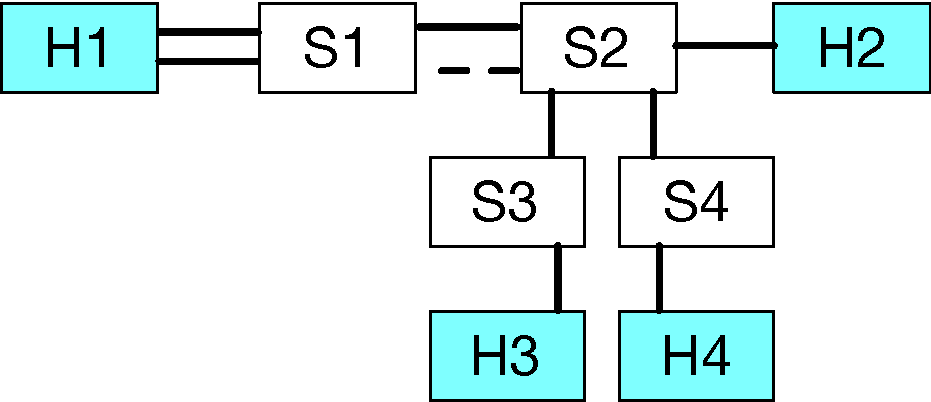
\includegraphics[width=0.3\paperwidth]{example_network.pdf}
  \caption{\label{fig:example-net}An example network consisting of four
    switches (S1-S4) and four hosts (H1-H4). Faulty links are shown as dashed lines.
    Each link is assumed to have capacity $R$ unless the link is faulty, in
    which case it has capacity $F < R$.  In this example, the failing link
    diminishes the bandwidth of H1.}
\end{figure}


\section{Background}
%Fat-tree topology, and port density.
%CorrOpt~\cite{Zhuo:2017:UMP:3098822.3098849}.
%Sources of failure: switch, transceivers, link medium.

\section{Design}
We assume that the underlying network is Ethernet, on which we implemented our
prototype.

\OurSys infers failing links and follows a policy on how to process frames
intended for those links. For all frames that cross failing links, we tag the
frames and use a \emph{forward error-correction} scheme: we complement frames
with extra parity frames to help the next hop recover frames that were lost in
transit.

In this section we describe \OurSys's policy choices for managing failing
links, and how the chosen policy is followed in the network.


\subsection{Traffic classification}
\label{sec:traffic-classification}
\OurSys is configured to have a (usually small) number of traffic classes,
which partitions the frames arriving at a switch. Encapsulated frames are
complemented with parity frames, forming \emph{blocks} that are sent across
the faulty link.
For each class $c$ we use a map $T: c \mapsto (k, h, t)$, where $k$ is the
number of frames in a block, $h$ is the number of parity frames sent for each
block, and $t$ is the timeout.
(When the encoding timer expires, the remaining frame spaces in a block are
zeroed out to provide padding.)
The values $(k, h, t)$ influence the latency with which frames belonging to $c$
cross the switch, as well the likely recovery of frames belonging to $c$. For
example, for interactive applications we would want to use a small $k$ and $t$.


\subsection{Link-failure management policy}
\label{sec:policy}
For each port the policy stipulates how to react if the link becomes faulty:
  \begin{itemize}
    \item Drop frames (i.e., disable the link); or
    \item Classify the frame, encode it, and forward.
  \end{itemize}
For the latter case, the policy specifies what are the traffic classifications,
and how does each classification map into parameters $(k, h, t)$.

In principle both the map $T$ (from~\S\ref{sec:traffic-classification}) and
the policy can be decided or changed while \OurSys is running, but for
consistency not while \OurSys is actually processing frames. In practice it is
resource-efficient to engineer to a limited set of choices to support.


\subsection{Execution}
\OurSys consists of three concurrent activities carried out for each port of a
switch:
\begin{itemize}
  \item \textbf{Link monitoring agent} attempts to infer link malfunction.
  \item \textbf{Sending proxy} processes frames before they are sent over a faulty link.
  \item \textbf{Receiving proxy} processes inbound \OurSys-tagged frames.
\end{itemize}

Frames to be sent over non-faulty links, and inbound frames that are not
\OurSys-tagged, are processed as normal by the switch. Otherwise outgoing frames
are processed by the Sending proxy prior to egress, and inbound frames by
the Receiving proxy after ingress.

\paragraph{\OurSys frame encapsulation}
Frames sent over faulty links are encapsulated as shown in Fig.~\ref{fig:format}.
The original frame is fully encapsulated, and the new header consists of the original source and destination addresses, as well as a custom EtherType for \OurSys.
After the Ethernet header we add a \OurSys tag, the field-sizes of which
are deployment-specific: the sizes we use in our implementation are specified
in~\S\ref{sec:implementation}.
The information in the \OurSys tag is sufficient to distinguish blocks in
non-bursty loss, as illustrated in Fig.~\ref{fig:example-loss}. If loss is
bursty then an additional small number of bits can be added to the tag to
mitigate against this, as shown in Fig.~\ref{fig:example-loss2}.

\paragraph{Link monitoring agent.}
  We continuosly poll network port counters to infer malfunctioning transceiver
  modules or links. This is done as in
  CorrOpt~\cite{Zhuo:2017:UMP:3098822.3098849}, but failure-inference is done
  locally on the switch, rather than remotely on a separate machine.
  Sometimes a switch cannot itself realise if one of its link is
  malfunctioning, since the malfunction would be inferrable from the adjacent
  element's counters (e.g., through an increase in frame errors). Thus switches
  might need to inform eachother about errors on the transmitting side. To do
  this we employ LLDP and use a custom TLV to signal to the receiving switch
  that the link (for traffic travelling in the opposite direction) is failing.
  The switch's monitoring would then follow the policy to disable the link or
  channel outgoing frames through the Sending proxy.


\paragraph{Receiving proxy.}
\OurSys-tagged frames are buffered as shown in Fig.~\ref{fig:example-decode},
and non-parity frames are untagged and forwarded immediately.
For each $c$, when the buffer is full, or its $t$ (relative to when the first
frame was buffered) expires, or a frame from a successive block arrives, then
decoding is triggered. Decoding consists of using the parity frames to
reconstruct the lost data frames; if no data frames have been lost then there
is no more work to be done for this block.

\paragraph{Sending proxy.}
The pseudo-code is shown in Algorithm~\ref{alg:sending}.
As with decoding, the encoding of a block (to produce parity frames) is
triggered when the block is full (all $k$ frames have been accounted for) or
$t$ for that $c$ expires (relative to when the first frame was inserted into
the block). Non-parity frames are tagged and forwarded immediately.

Due to its operation, the sending proxy can cause congestion at egress.
For example, if $k = h$, and we are receiving traffic bound for
a faulty link at rate $R$, then we would need to send at $2R$ at each interval
of $k$ incoming frames, at which time the sending proxy produces $h$ additional
frames for output. We simply drop new frames that cannot be put onto the link
fast enough (i.e., before they are placed into a block). This lack of capacity
is communicated by the $\mathit{busy}(c)$ predicate in
Algorithm~\ref{alg:sending}, which indicates that the FEC computation is
ongoing, or its results are still being serialised onto the medium. This loss
will communicate to higher-layer protocols that congestion is occurring (both
due to the link capacity being reduced, and because of the extra overhead of
sending the parity frames), and the end-hosts network stacks can react to this
congestion as they normally would.

\begin{algorithm}
\SetAlgoLined
\SetKwInOut{Input}{input}\SetKwInOut{Output}{output}
\Input{frame to be forwarded}
\Output{forwarding decision}
\uIf(\tcc*[h]{Link has been disabled}){policy = drop}{
drop frame\;
}\Else(\tcc*[h]{Use FEC}){
  $c = P(\mathrm{frame})$ \tcc*[r]{Classify the frame}
  \uIf(\tcc*[h]{Block is being sent}){busy(c)}{
drop frame\;
}\Else{
  $\overline{\mathrm{frame}}$ = encapsulate($c, \mathrm{frame}$)\;
  addToBlock($c$, $\overline{\mathrm{frame}}$)\;
  forward $\overline{\mathrm{frame}}$\;
}
}
\caption{\label{alg:sending}Sending proxy}
\end{algorithm}

%\begin{algorithm}
%\SetAlgoLined
%\SetKwFunction{FName}{addToBlock}%
%\SetKwProg{Proc}{Procedure}{\string:}{}
%\Proc{\FName{c, frame}}{
%\uIf(\tcc*[h]{Link has been disabled}){policy = drop}{
%drop frame
%}\Else(\tcc*[h]{Use FEC}){
%  $c = P(\mathrm{frame})$\;
%  addToBlock($c$, frame)\;
%}
%}
%\caption{\label{alg:sending}Adding a frame to a block for class $c$}
%\end{algorithm}

\begin{figure}
  \centering
  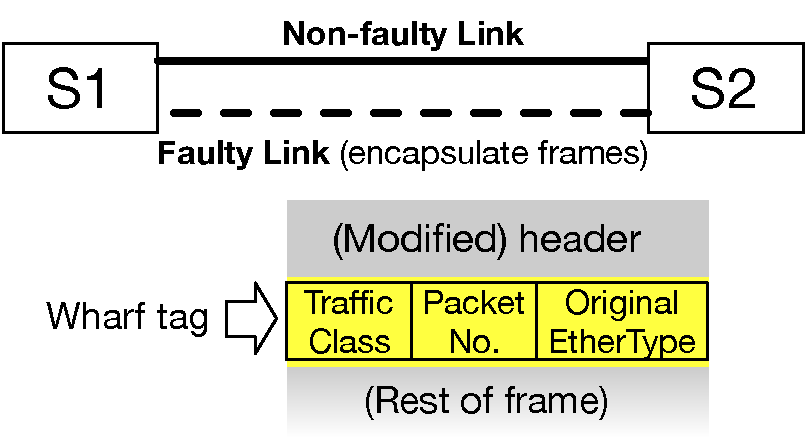
\includegraphics[width=0.3\paperwidth]{header_format.pdf}
  \caption{\label{fig:format}Switches can have multiple links between them.
  Traffic on faulty links is encapsulated as shown above: the frame's EtherType
  is moved inside the \OurSys tag (and later moved back after the frame crosses
  the link), the frame's EtherType is changed to \OurSys, and the frame is
  classified to a particular Traffic Class and given a transient link-local
  identifier: these are shown as $c$ and $n$ respectively in
  Fig.~\ref{fig:example-loss}.}
\end{figure}

\begin{figure}
  \centering
  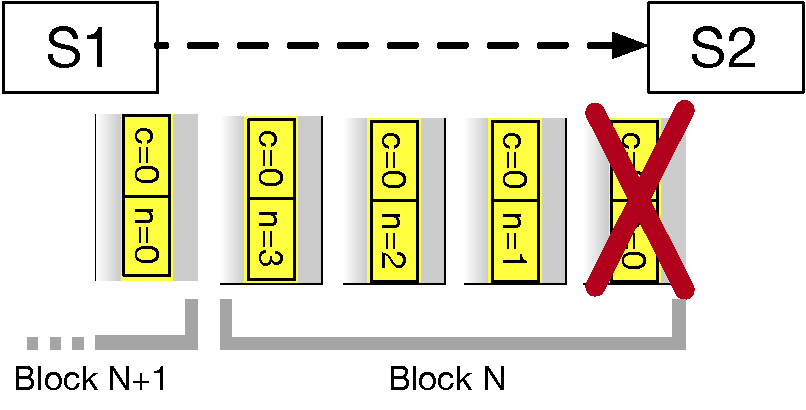
\includegraphics[width=0.4\paperwidth]{loss_example.pdf}
  \caption{\label{fig:example-loss}The expectation for strictly monotonic frame
  number $n$ ensures that we can distingush successive blocks. Note that frame
  reordering is not possible because they are being sent over the same link,
  and their processing is sequential across that link.}
\end{figure}

\begin{figure}
  \centering
  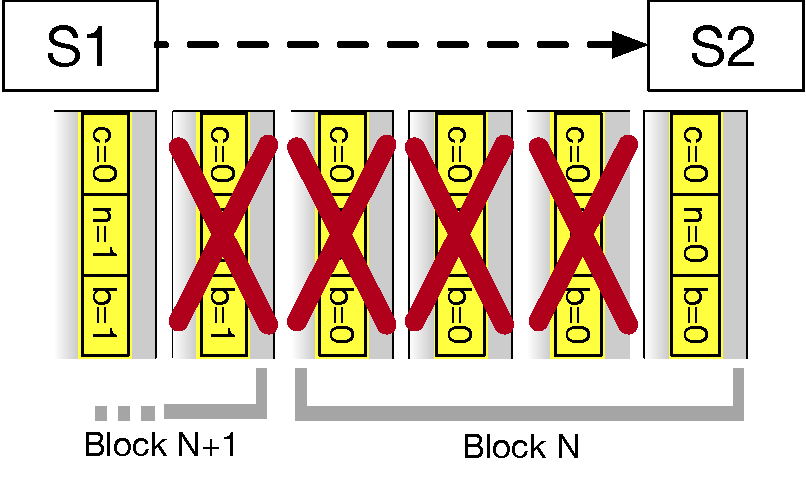
\includegraphics[width=0.4\paperwidth]{loss_example2.pdf}
  \caption{\label{fig:example-loss2}To mitigate bursty loss a block counter is added.}
\end{figure}

\begin{figure}
  \centering
  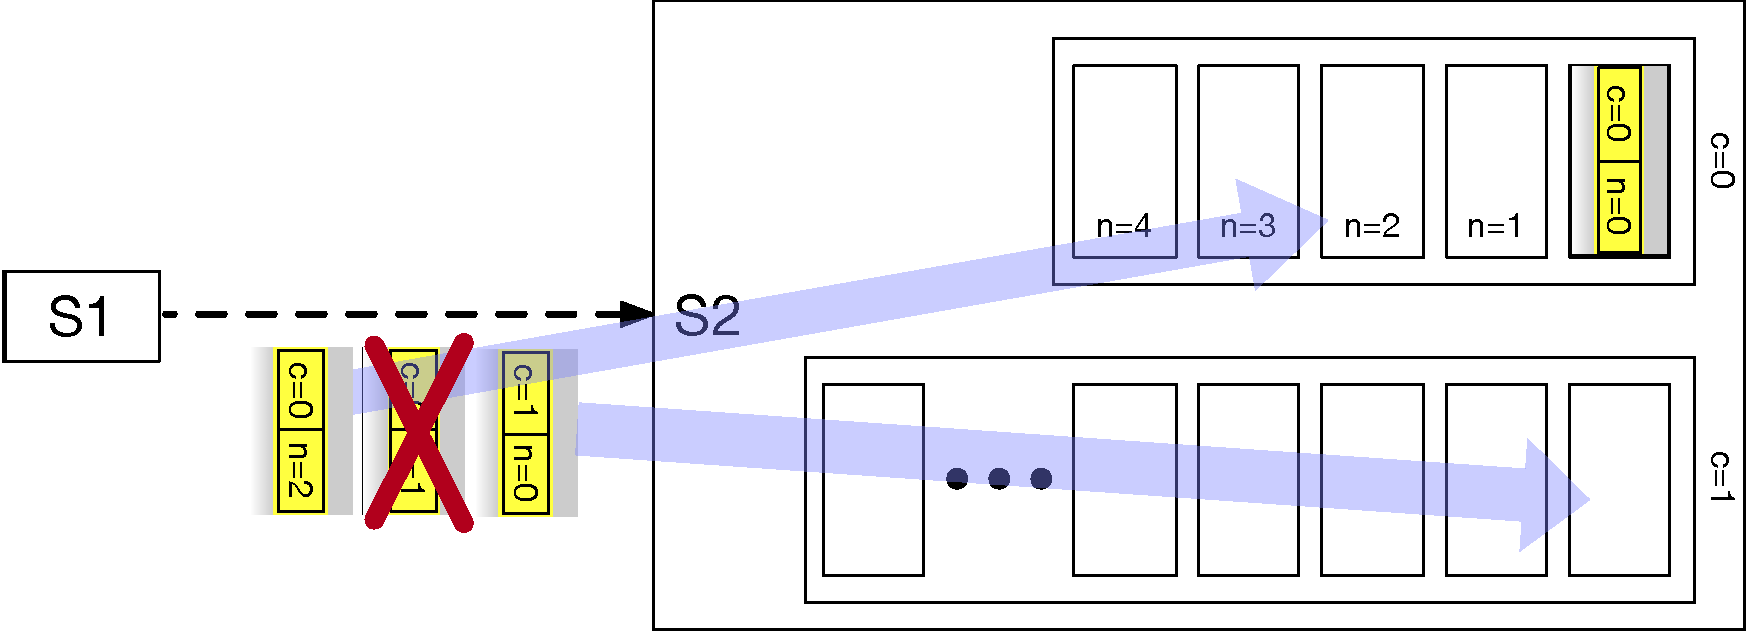
\includegraphics[width=0.4\paperwidth]{decode_example.pdf}
  \caption{\label{fig:example-decode}Prior to decoding each block is mapped to the buffer for its traffic class.}
\end{figure}


\section{Implementation}
\label{sec:implementation}
\section{Evaluation}
We evaluate \OurSys using different types of traffic to measure its improvement
to application-level behaviour in the presence of lossy links.

%We run \OurSys in 3 configurations: outside the switch, on the switch, and in the switch.
%Time how quickly \OurSys reacts to failing links.

\section{Conclusion}

\bibliographystyle{ACM-Reference-Format}
\bibliography{paper}

\end{document}
